%!TEX root=main.tex

\section{Related Work} \label{sec:related_work}

\subsection{Uncertainty in Neural Networks}
Neural networks have achieved state-of-the-art results on estimating human intent~\cite{Vemula2017, Alahi2016}. However, one fundamental difference in human and neural network reasoning is uncertainty. Neural networks normally predict a mean prediction value and can fail over-confidently on novel data. Humans, in comparison, would reveal their uncertainty saying \textit{I have never seen this behavior before, hence I do not know how to predict the behavior}. To give the neural networks a similar notion of uncertainty and \textit{know what they don't know}, we have explored the recent field uncertainty-aware neural networks. 

Bayesian Neural Networks reason about predictive uncertainty by keeping track of a distribution for each network's parameter~\cite{MacKay1992, Neal1996}. However, they are computationally intractable due to the expensive calculation of the Bayesian posterior. Even approximate methods, such as Markov Chain Monte Carlo or variational methods, come with extensive computational cost~\cite{Louizos2016, Graves2011, Springenberg_2016}. Other works, proposes MC-Dropout~\cite{Gal2015}: the activation of Dropout~\cite{Dropout2014} during test as approximate Bayesian inference in deep Gaussian processes. However, uncertainty estimates with MC-Dropout have shown to be overconfident on novel data~\cite{Osband2016, Lakshmi2016}. 

Alternative works proposes the Bootstrapping as an approximation of model uncertainty in neural networks~\cite{Osband2016, Lakshmi2016}. Intuitively, an ensemble of randomly initialized models is trained on overlapping samples of a training dataset and during test the sample variance of predictions indicates the ensemble uncertainty. The predictions of each model will be similar for data points that have often occurred in the training set and differ for data points that have only occurred in one sample of the training set or not occurred at all. 

\subsection{Intuitive physics understanding}
This work was inspired by \cite{Lerer, Bramley2017} who explored how to simulate our intuition about physics, and did so using deep feed-forward models to learn intuitive physics.

\begin{figure}[]
	\begin{subfigure}[]{1\linewidth}
		\centering
		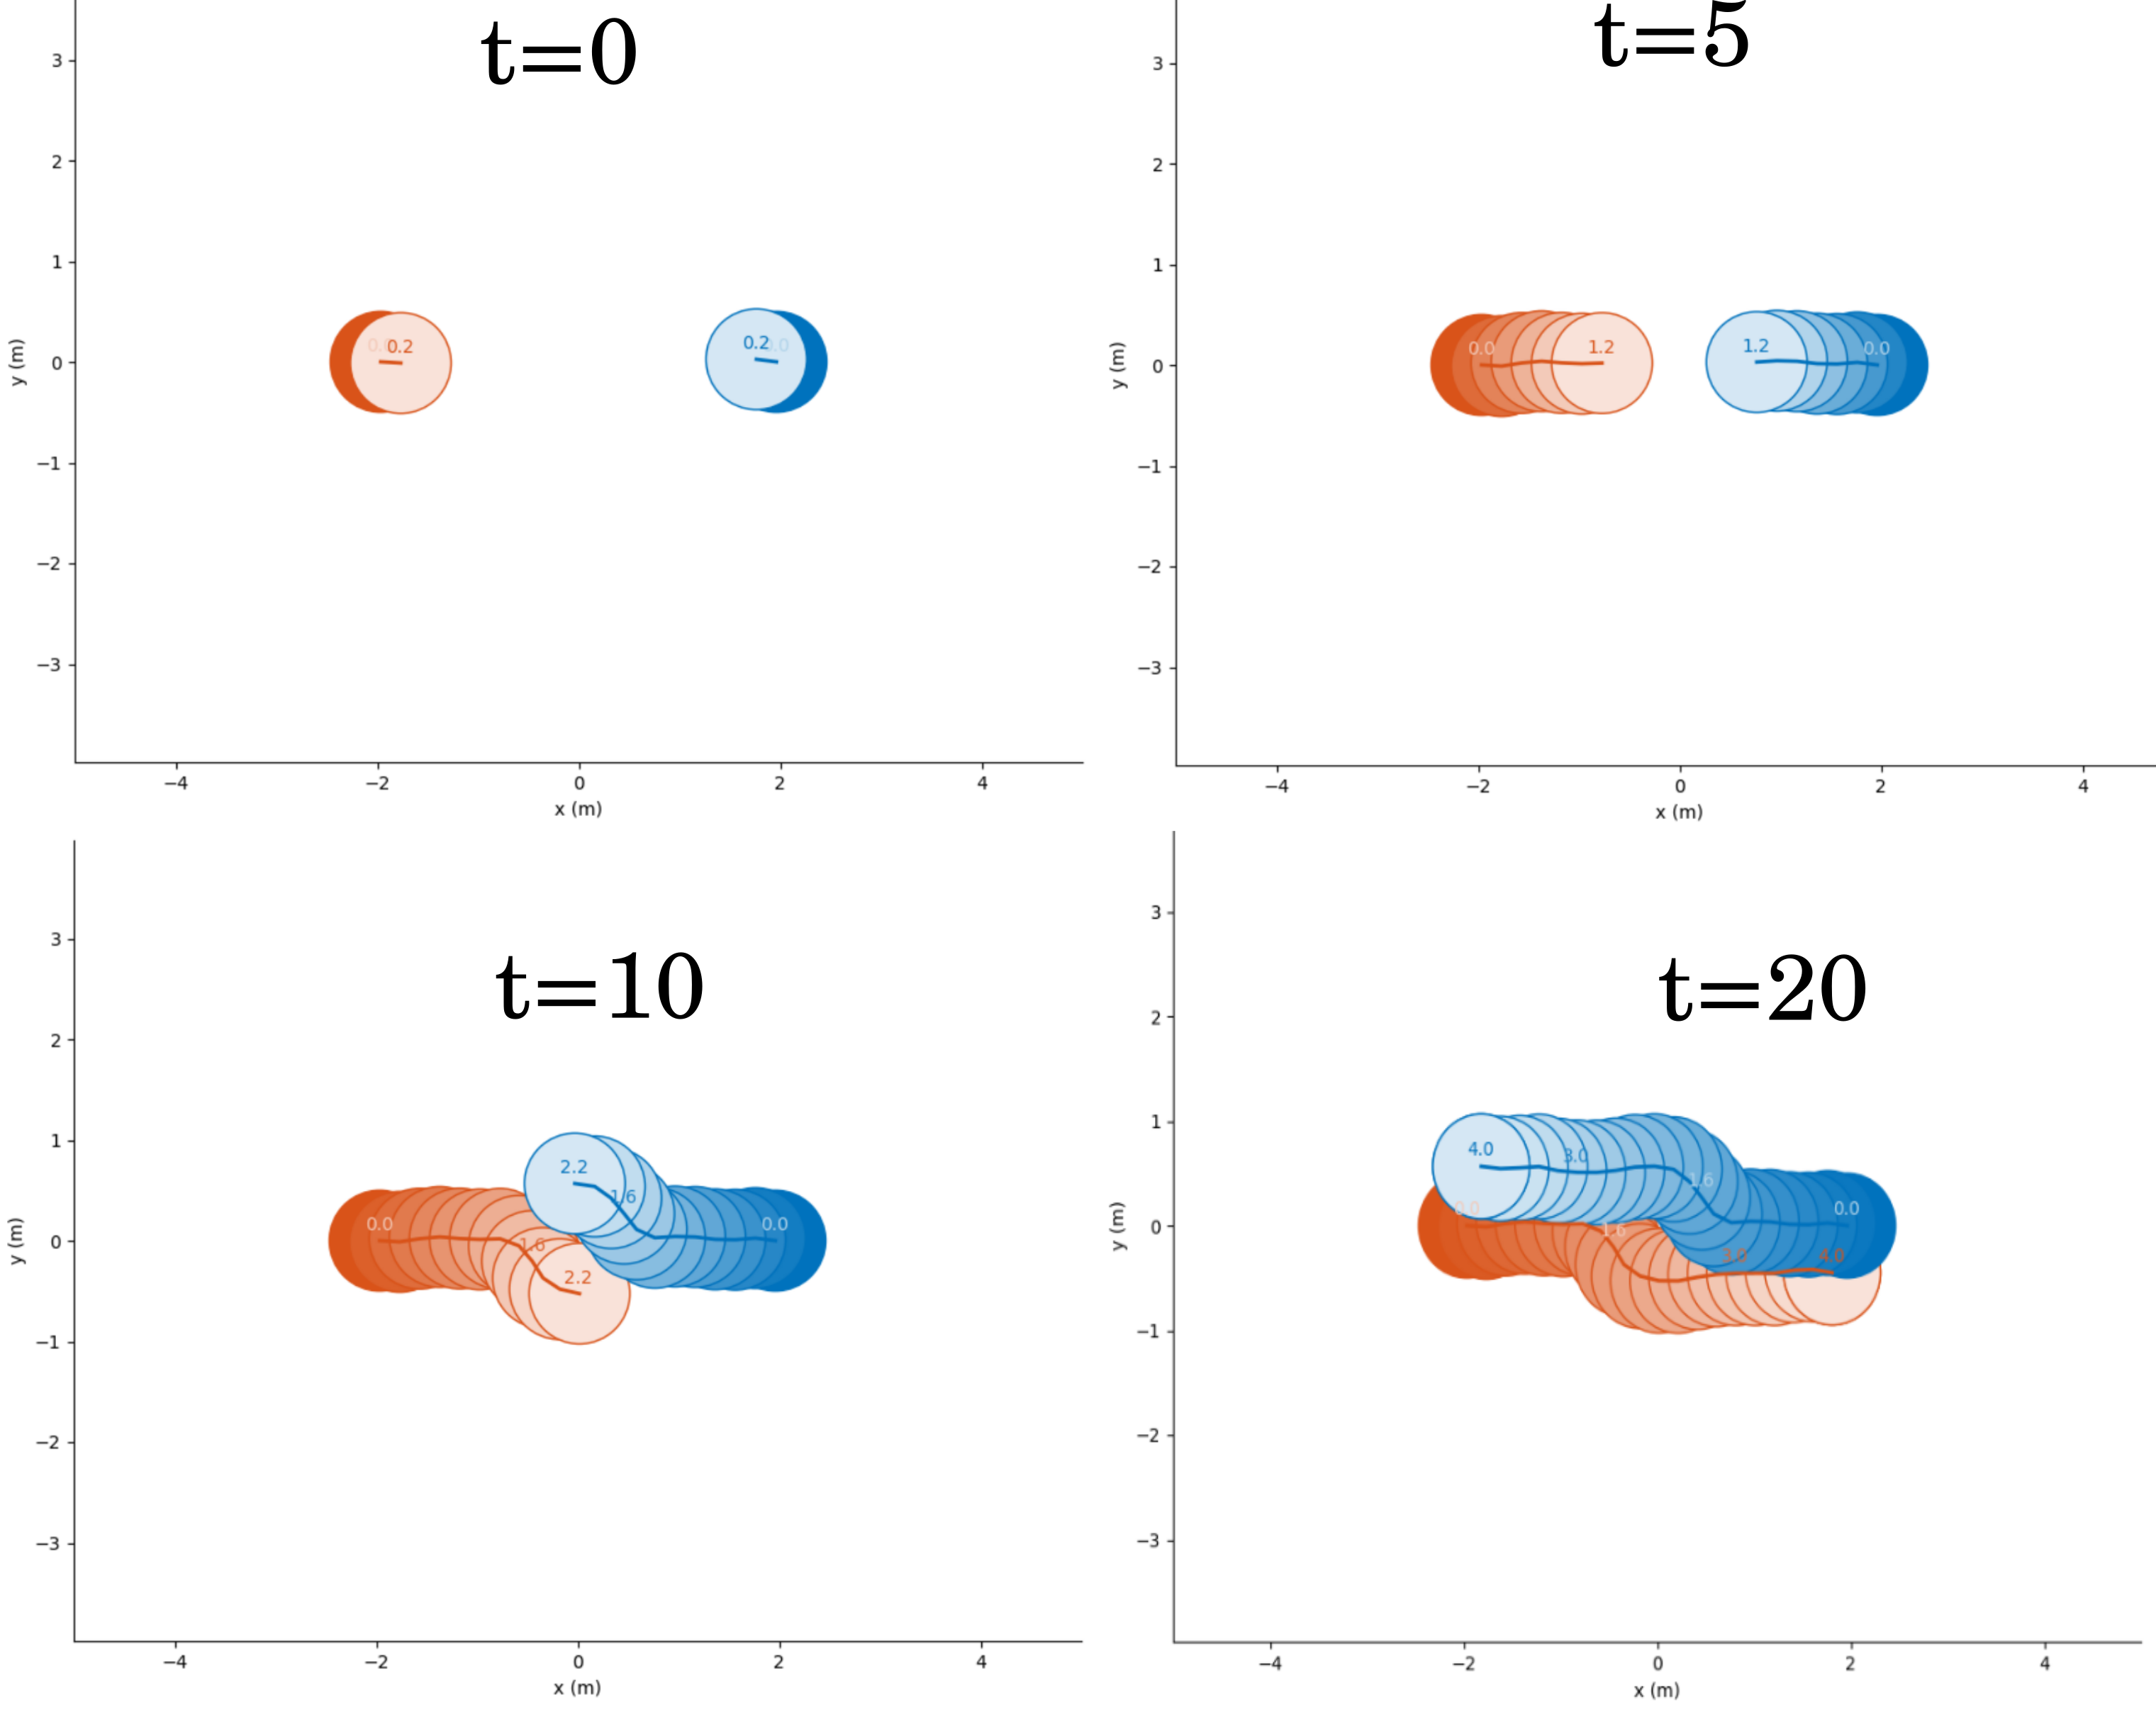
\includegraphics[width=0.95\linewidth]{figures/sim_no_coll.png}
		\caption{Example trajectory with no collision.}
		\label{fig:sim_no_coll}
	\end{subfigure}
	\\
	\begin{subfigure}[]{1\linewidth}
		\centering
		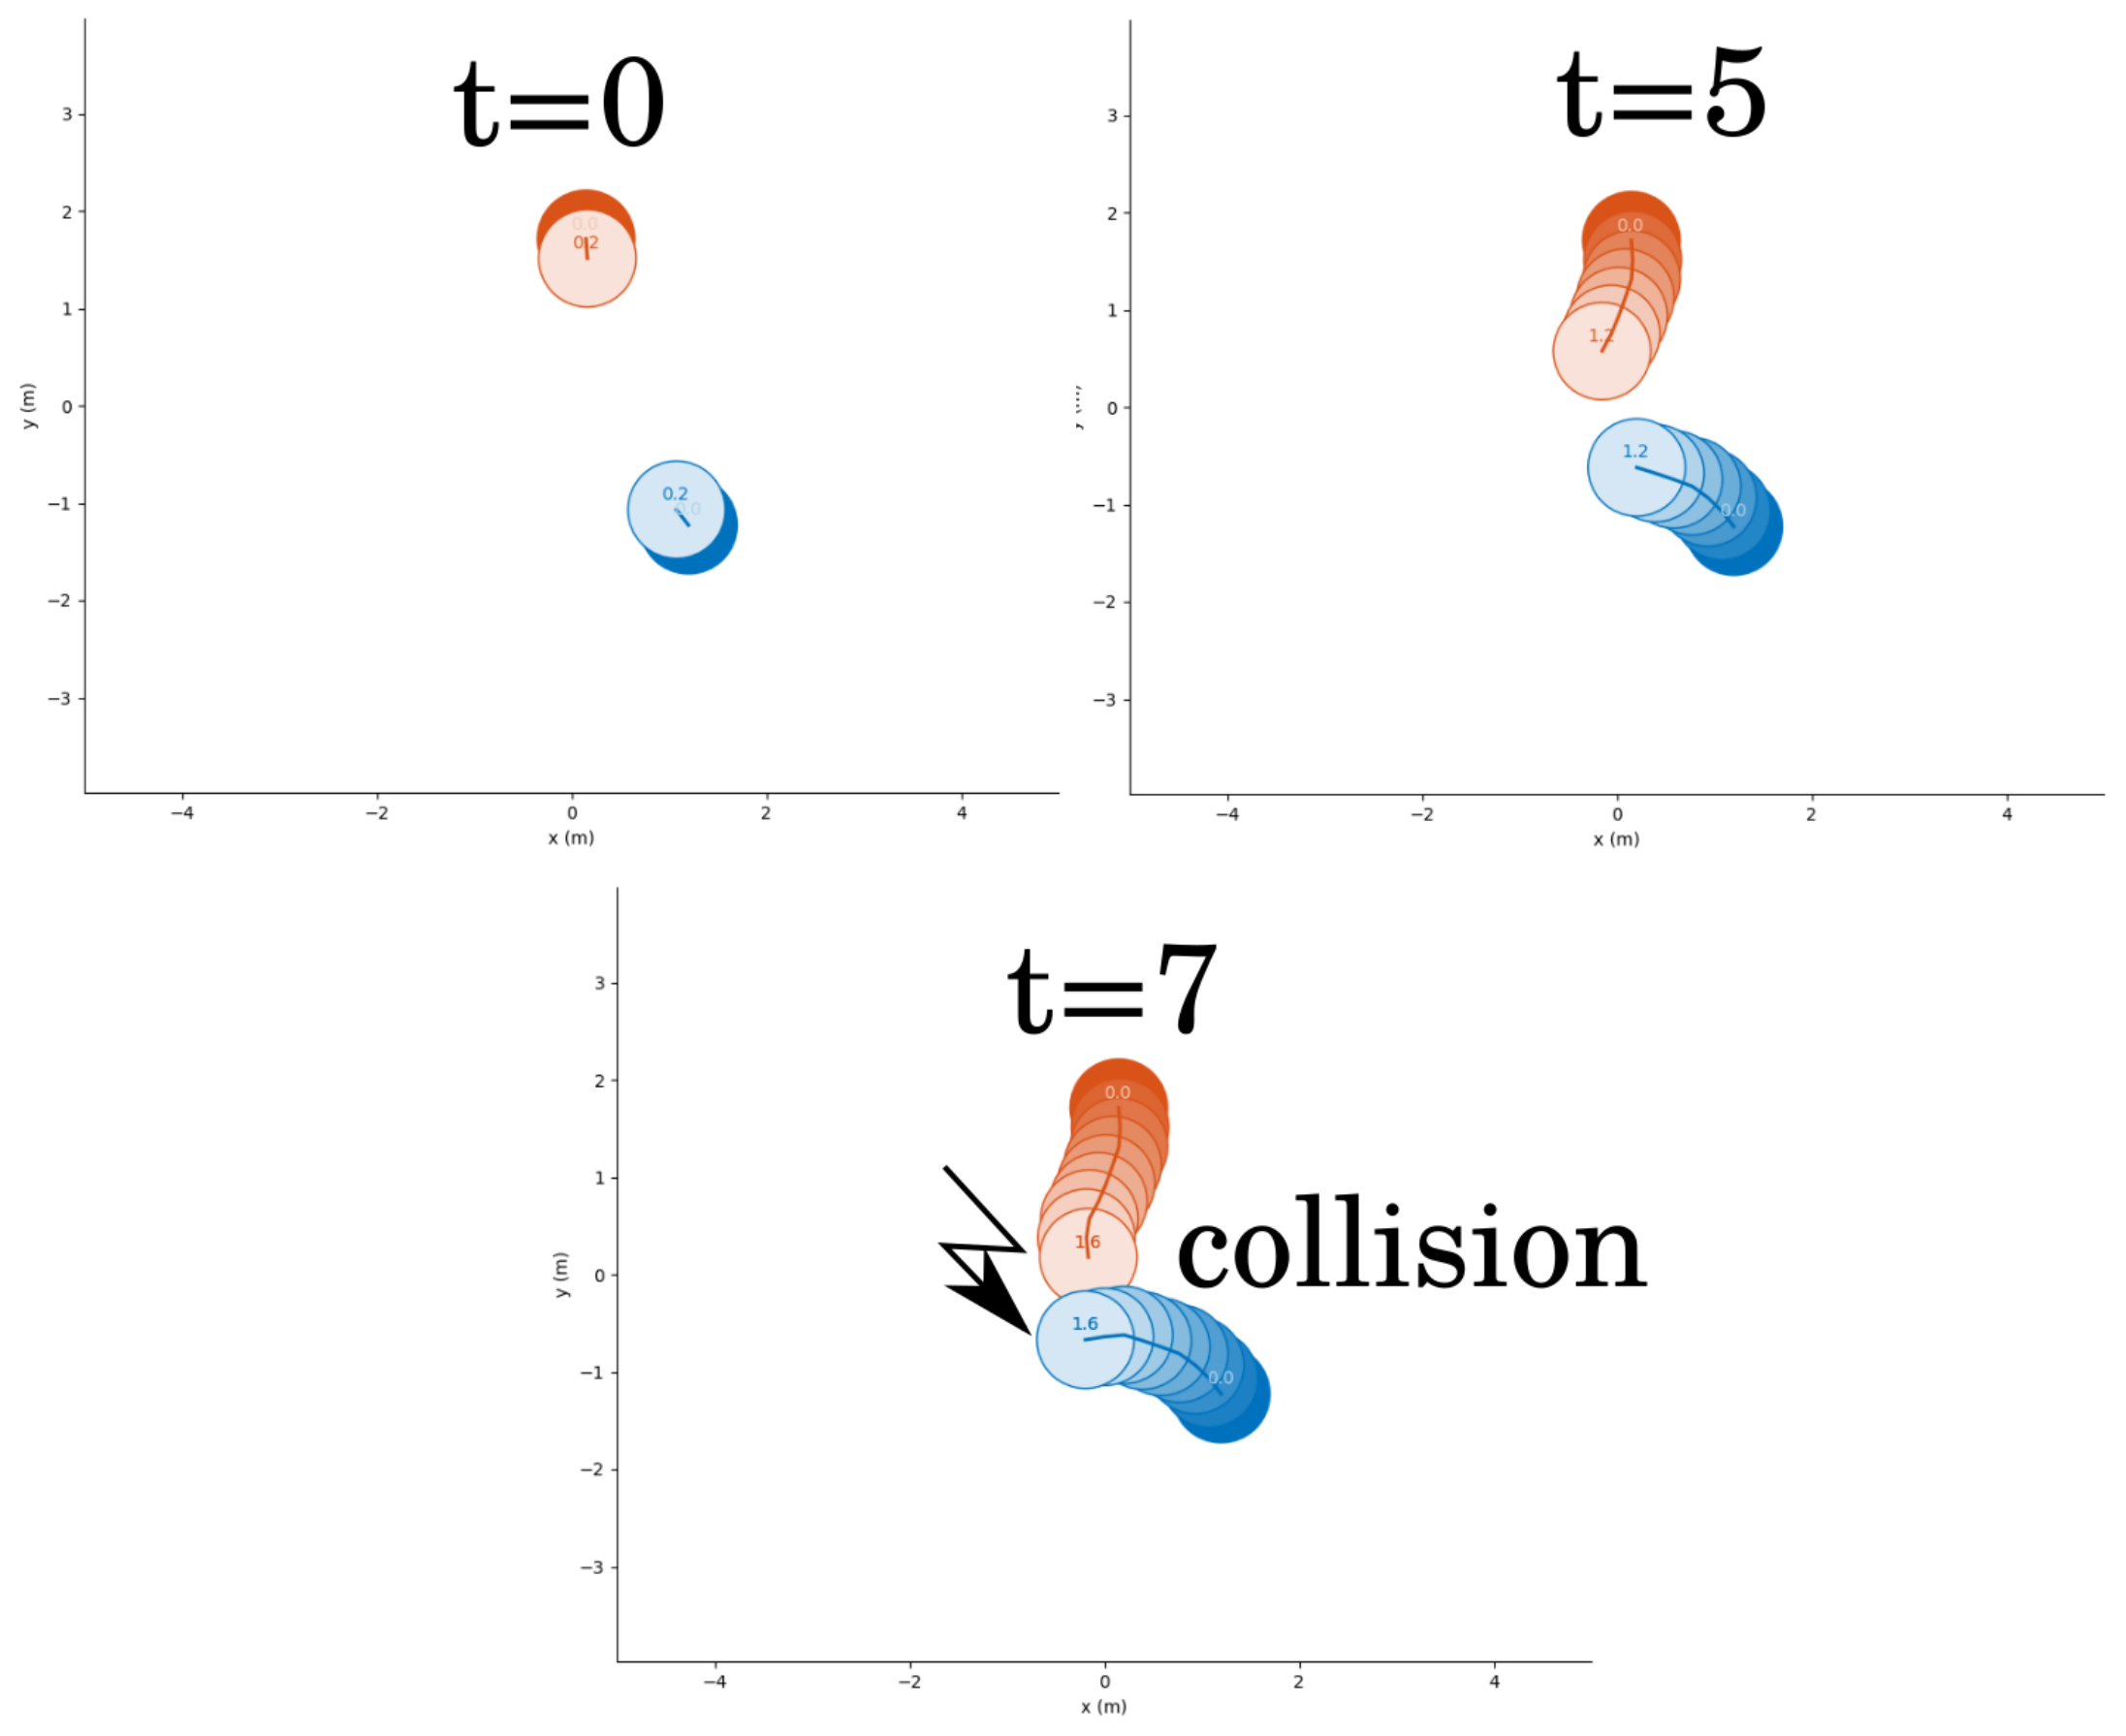
\includegraphics[width=0.95\linewidth]{figures/sim_coll.png}
		\caption{Example trajectory with collision.}
		\label{fig:sim_coll}
	\end{subfigure}
    \caption{Pedestrian Simulation. In the beginning of each episode, the pedestrian simulation randomly spawns two pedestrians (dark orange and blue circle) at time $t=0$ at a random $x-y$ position. The simulation uses a pedestrian dynamics model to propagate the positions over time. The  bird's eye perspective of the pedestrian positions is displayed. At each time step the updated pedestrian position is plotted whose color becomes lighter over time. In ~\cref{fig:sim_no_coll} two pedestrians avoid each other and in~\cref{fig:sim_coll} two pedestrians collide.} 
    \label{fig:ped_sim}
\end{figure}
